%% Template for MLP Coursework 2 / 6 November 2017

%% Based on  LaTeX template for ICML 2017 - example_paper.tex at
%%  https://2017.icml.cc/Conferences/2017/StyleAuthorInstructions

\documentclass{article}

\usepackage[T1]{fontenc}
\usepackage{amssymb,amsmath}
\usepackage{txfonts}
\usepackage{microtype}

% For figures
\usepackage{graphicx}
\usepackage{subfigure}

% For citations
\usepackage{natbib}

% For algorithms
\usepackage{algorithm}
\usepackage{algorithmic}

% the hyperref package is used to produce hyperlinks in the
% resulting PDF.  If this breaks your system, please commend out the
% following usepackage line and replace \usepackage{mlp2017} with
% \usepackage[nohyperref]{mlp2017} below.
\usepackage{hyperref}
\usepackage{url}
\urlstyle{same}

% Packages hyperref and algorithmic misbehave sometimes.  We can fix
% this with the following command.
\newcommand{\theHalgorithm}{\arabic{algorithm}}


% Set up MLP coursework style (based on ICML style)
\usepackage{mlp2017}
\mlptitlerunning{MLP Coursework 2 (\studentNumber)}
\bibliographystyle{icml2017}


\DeclareMathOperator{\softmax}{softmax}
\DeclareMathOperator{\sigmoid}{sigmoid}
\DeclareMathOperator{\sgn}{sgn}
\DeclareMathOperator{\relu}{relu}
\DeclareMathOperator{\lrelu}{lrelu}
\DeclareMathOperator{\elu}{elu}
\DeclareMathOperator{\selu}{selu}
\DeclareMathOperator{\maxout}{maxout}

%% You probably do not need to change anything above this comment

%% REPLACE this with your student number
\def\studentNumber{s1781323}

\begin{document}

\twocolumn[
\mlptitle{MLP Coursework 2: Learning rules, BatchNorm, and ConvNets}

\centerline{\studentNumber}

\vskip 7mm
]

\begin{abstract}
% The abstract should be 100--200 words long,  providing a concise summary of the contents of your report.
This coursework is the experiment on batch normalization and CNN. At first, we show the result on a baseline model, then test models with different learning rules, batch normalization, CNN, and so on with the explanation of these concepts.

Compared to stochastic gradient descent, the optimizers called RMSProp and Adam converges faster and more property, and it is beneficial for the neural network. Dropout is the method to prevent overfitting. It may worsen the accuracy depend on the usage, but it improves generalization ability. Batch normalization normalizes data in each layer and enhances performance dynamically. CNN increases the performance as well.

The best model in this paper is the combination of batch normalization and CNN. However, it takes the enormous computational cost. This is another critical problem in this field.
\end{abstract}

\section{Introduction}
\label{sec:intro}
The aim of this coursework is to further explore the classification of images of handwritten digits using neural networks. Recently we see so many article on new techniques and how they bring breakthrough to this industory. In this report, we test several learning rules, batch normalization, and convolution networks and techniques including dropout.

In this report we use EMNIST (Extended MNIST) Balanced dataset, https://www.nist.gov/itl/iad/ image-group/emnist-dataset [Cohen et al., 2017]. EMNIST extends MNIST by including images of handwritten letters (upper and lower case) as well as handwritten digits. Both EMNIST and MNIST are extracted from the same underlying dataset, referred to as NIST Special Database 19. Both use the same conversion process resulting in centred images of dimension 28 X 28. Although there are 62 potential classes for EMNIST (10 digits, 26 lower case letters, and 26 upper case letters).  The expected accuracy rates are lower for EMNIST than for MNIST. We use a reduced label set of 47 different labels. We use 100,000 data for training, and 15800 data for validation.


\section{Baseline systems}
For baseline system, we construct a neuralnetwork with two hidden layers. We use ReLU function as activation, and SGD as learning rule. The hidden units of each layers are 100, and the last output is 47.
After the section, we add components or replace learning rules.

The lerning rate is 0.001.
\begin{figure}[h]
\vskip 5mm
\begin{center}
\centerline{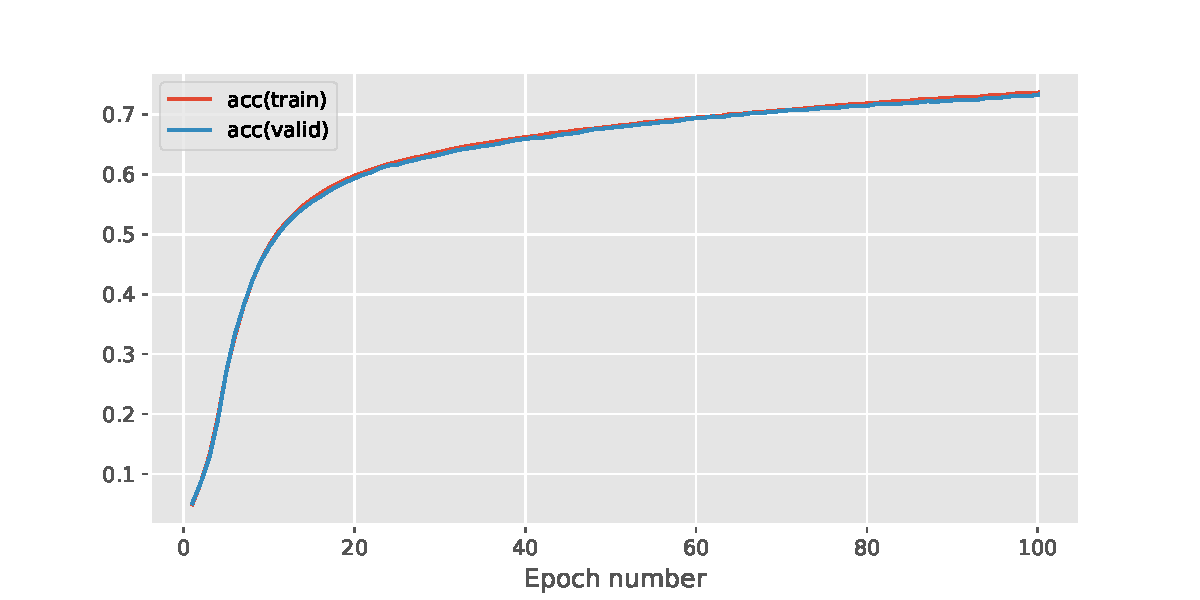
\includegraphics[width=\columnwidth]{a.pdf}}
\caption{Accuracy of baseline system.
Accuracy of train dataset:0.737
Accuracy of valid dataset:0.733
}
\end{center}
\vskip -5mm
\end{figure}

Also we implement three hidden layers because it gives more parameters. As a result the accuracy improves.
\begin{figure}[h]
\vskip 5mm
\begin{center}
\centerline{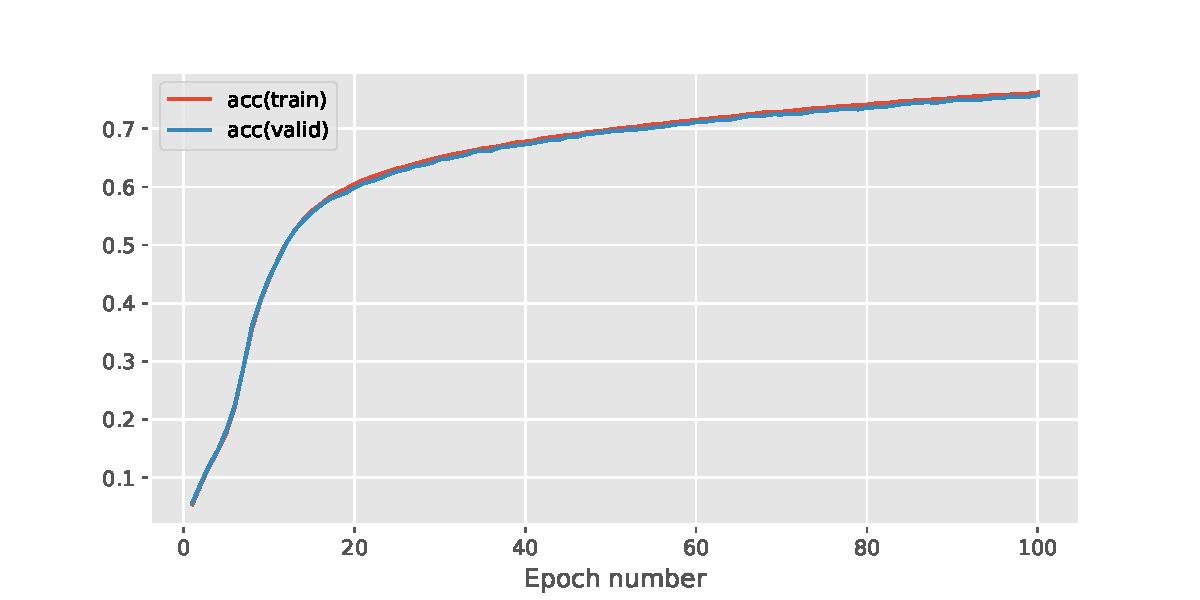
\includegraphics[width=\columnwidth]{b.pdf}}
\caption{Accuracy of models with three hidden layers.
Accuracy of train dataset:0.762
Accuracy of valid dataset:0.758
}
\end{center}
\vskip -5mm
\end{figure}

These result show that the trained model in not overfitted because the accuracy of both train and validation sets are close.

Finally for this section, we applied dropout technique to the last affine layer in the baseline model. The input optimal probability of retention(p) is 0.5.
Dropout is the technique to privent overfit. While training, dropout stop some units stochastically and operate forward pass and bachpropagation. This method reduce the parameters while training, so it prevents overfit, however, this may decrease the accuracy of prediction.
The result on figure 3 shows that the difference of accuracies reduces. Also the learning curve goes smooth. However, this method worsen the accuracy. It is hard to find appropriate p and model to use dropout technique.

\begin{figure}[h]
\vskip 5mm
\begin{center}
\centerline{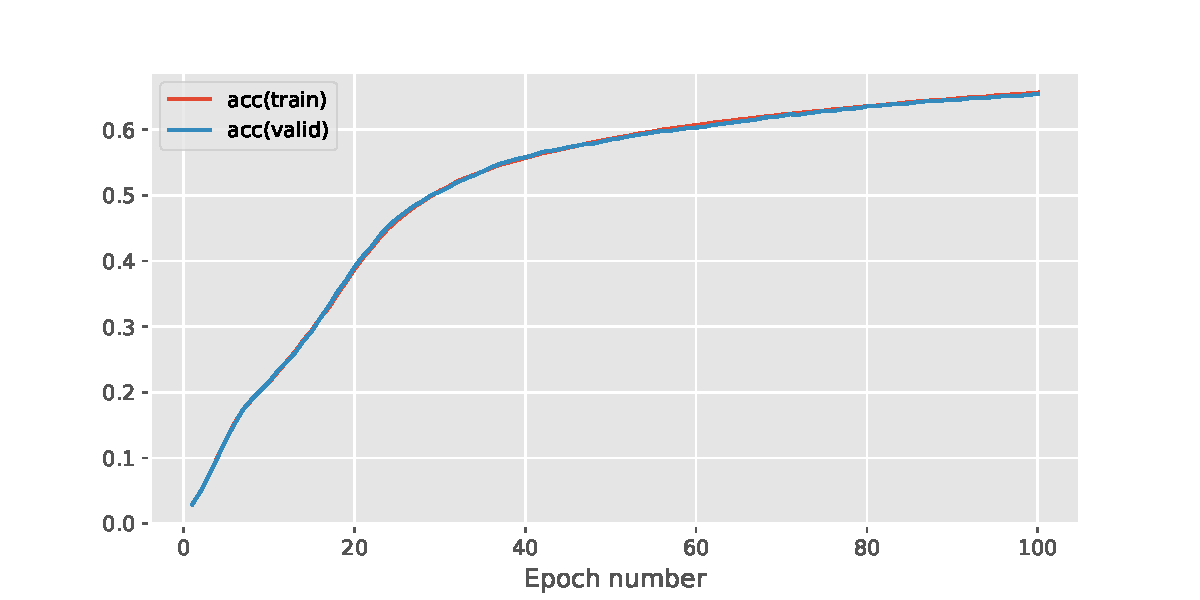
\includegraphics[width=\columnwidth]{c.pdf}}
\caption{Accuracy of models with three hidden layers.
Accuracy of train dataset:0.657
Accuracy of valid dataset:0.655
}

\end{center}
\vskip -5mm
\end{figure}
% In this section you should report your baseline experiments for EMNIST.  No need for theoretical explanations of things covered in the course, but should you go beyond what was covered please explain what you did with references to relevant paper(s) if appropriate.   In this section you should aim to cover the both the ``what'' and the ``why'': \emph{what} you did, giving sufficient information (hyperparameter settings, etc.) so that someone else (e.g. another student on the course) could reproduce your results; and \emph{why} you performed the experiments you are reporting - what you are aiming to discover what is the motivation for the particular experiments you undertook. You should also provide some discussion and interpretation of your results.
%
% As before, your experimental sections should include graphs (for instance, figure~\ref{fig:sample-graph}) and/or tables (for instance, table~\ref{tab:sample-table})\footnote{These examples were taken from the ICML template paper.}, using the \verb+figure+ and \verb+table+ environments, in which you use \verb+\includegraphics+ to include an image (pdf, png, or jpg formats).  Please export graphs as
% \href{https://en.wikipedia.org/wiki/Vector_graphics}{vector graphics}
% rather than \href{https://en.wikipedia.org/wiki/Raster_graphics}{raster
% files} as this will make sure all detail in the plot is visible.
% Matplotlib supports saving high quality figures in a wide range of
% common image formats using the
% \href{http://matplotlib.org/api/pyplot_api.html\#matplotlib.pyplot.savefig}{\texttt{savefig}}
% function. \textbf{You should use \texttt{savefig} rather than copying
% the screen-resolution raster images outputted in the notebook.} An
% example of using \texttt{savefig} to save a figure as a PDF file (which
% can be included as graphics in a \LaTeX document is given in the coursework 1 document.
%
% If you need a figure or table to stretch across two columns use the \verb+figure*+ or \verb+table*+ environment instead of the \verb+figure+ or \verb+table+ environment.  Use the \verb+subfigure+ environment if you want to include multiple graphics in a single figure.
%
% \begin{figure}[tb]
% \vskip 5mm
% \begin{center}
% \centerline{\includegraphics[width=\columnwidth]{icml_numpapers.pdf}}
% \caption{Historical locations and number of accepted papers for International
%   Machine Learning Conferences (ICML 1993 -- ICML 2008) and
%   International Workshops on Machine Learning (ML 1988 -- ML
%   1992). At the time this figure was produced, the number of
%   accepted papers for ICML 2008 was unknown and instead estimated.}
%
% \end{center}
% \vskip -5mm
% \end{figure}
%
% \begin{table}[tb]
% \vskip 3mm
% \begin{center}
% \begin{small}
% \begin{sc}
% \begin{tabular}{lcccr}
% \hline
% \abovespace\belowspace
% Data set & Naive & Flexible & Better? \\
% \hline
% \abovespace
% Breast    & 95.9$\pm$ 0.2& 96.7$\pm$ 0.2& $\surd$ \\
% Cleveland & 83.3$\pm$ 0.6& 80.0$\pm$ 0.6& $\times$\\
% Glass2    & 61.9$\pm$ 1.4& 83.8$\pm$ 0.7& $\surd$ \\
% Credit    & 74.8$\pm$ 0.5& 78.3$\pm$ 0.6&         \\
% Horse     & 73.3$\pm$ 0.9& 69.7$\pm$ 1.0& $\times$\\
% Meta      & 67.1$\pm$ 0.6& 76.5$\pm$ 0.5& $\surd$ \\
% Pima      & 75.1$\pm$ 0.6& 73.9$\pm$ 0.5&         \\
% \belowspace
% Vehicle   & 44.9$\pm$ 0.6& 61.5$\pm$ 0.4& $\surd$ \\
% \hline
% \end{tabular}
% \end{sc}
% \end{small}
% \caption{Classification accuracies for naive Bayes and flexible
% Bayes on various data sets.}
% \label{tab:sample-table}
% \end{center}
% \vskip -3mm
% \end{table}

\section{Learning rules}
In this section we introduce RMSProp and Adam with gradient descent, and then compare with SGD rule.

{\bf RMSProp:}
RMSProp is presented by Hinton in the Coursera course, and this is a stochastic gradient descent version of RProp, normalised by a moving average of the squared gradient.
\begin{equation}
    \begin{align}
        S_i(t) = \beta S_i(t-1) + (1 - \beta) g_i(t)^2  \\
        \Delta w_i(t) = -\frac{\eta}{\sqrt{S_i(t)}+ \epsilon}g_i(t)
    \end{align}
\end{equation}
$\beta$ is usually 0.9. $\eta$ is learning rate and 0.001 is appropriate. $\g$ is the gradient of $i$th parameter.


{\bf Adam:}
Adam is presented by Kingma and Ba. In addition to storing an exponentially decaying average of past squared gradients like RMSprop, Adam also keeps an exponentially decaying average of past gradients similar to momentum:
\begin{equation}
    \begin{align}
        m_i(t) = \beta_1 m_i(t-1) + (1-\beta)g_i(t) \\
        v_i(t) = \beta_2 v_i(t-1) + (1-\beta_2)g_i(t)^2 \\
        \hat{m_i(t)} = \frac{m_i(t)}{1 - \beta_1 ^ t} \\
        \hat{v_i(t)} = \frac{v_i(t)}{1-\beta_2^t} \\
        \Delta w_i(t) = -\frac{\eta}{\sqrt{\hat{v_i(t)}}+ \epsilon}\hat{m_i(t)}
  \end{align}
 \end{equation}
$\beta_1$ is usually 0.9. $\beta_2$ is 0.999 $\eta$ is learning rate and 0.001 is appropriate. $\g$ is the gradient of $i$th parameter.

% \begin{algorithm}[ht]
% \begin{algorithmic}
%    \STATE {\bfseries Input:} data $x_i$, size $m$
%    \REPEAT
%    \STATE Initialize $noChange = true$.
%    \FOR{$i=1$ {\bfseries to} $m-1$}
%    \IF{$x_i > x_{i+1}$}
%    \STATE Swap $x_i$ and $x_{i+1}$
%    \STATE $noChange = false$
%    \ENDIF
%    \ENDFOR
%    \UNTIL{$noChange$ is $true$}
% \end{algorithmic}
%   \caption{Bubble Sort}
%   \label{alg:example}
% \end{algorithm}
The learning rule in baseline is Stochastic gradient descent (SGD). However, Dauphin et al. argues that saddle points are usually surrounded by a plateau of the same error, which makes it notoriously hard for SGD to escape as the gradient is close to zero in all dimensions.

The results is on figure 4 and 5 and Table 1.

\begin{table}[h]
\vskip 3mm
\begin{center}
\begin{small}
\begin{sc}
\begin{tabular}{lcccr}
\hline
\abovespace\belowspace
&acc(train) & acc(val) & error(train) & error(val) \\
\hline
\abovespace
SGD     & 0.737      & 0.733           & 0.919        & 0.936             \\ \hline
RMSProp & 0.944      & 0.809           & 0.135        & 1.37              \\ \hline
Adam    & 0.943      & 0.812           & 0.138        & 1.20              \\
\hline
\end{tabular}
\end{sc}
\end{small}
\caption{Accuracy and mean square error of models with three different learning rules. Error is mean square error. Model is based on baseline.}
\label{tab:sample-table}
\end{center}
\vskip -3mm
\end{table}

\begin{figure}[h]
\vskip 5mm
\begin{center}
\centerline{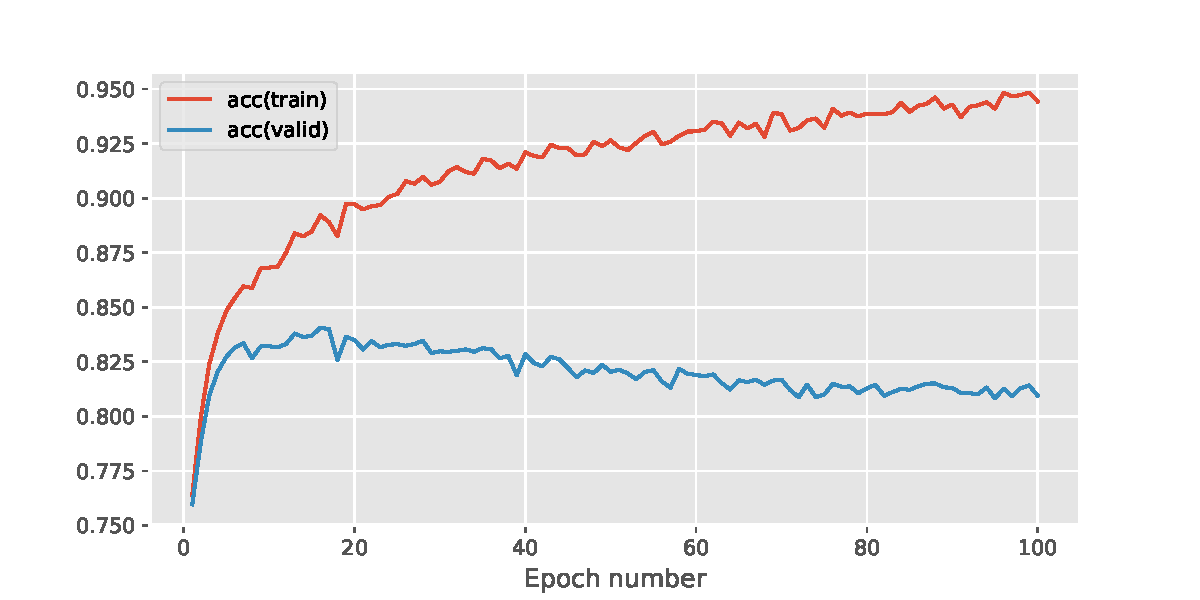
\includegraphics[width=\columnwidth]{d.pdf}}
\caption{Accuracy of models with RMSProp learning rule.
Accuracy of train dataset:0.944
Accuracy of valid dataset:0.809
}

\end{center}
\vskip -5mm
\end{figure}

\begin{figure}[h]
\vskip 5mm
\begin{center}
\centerline{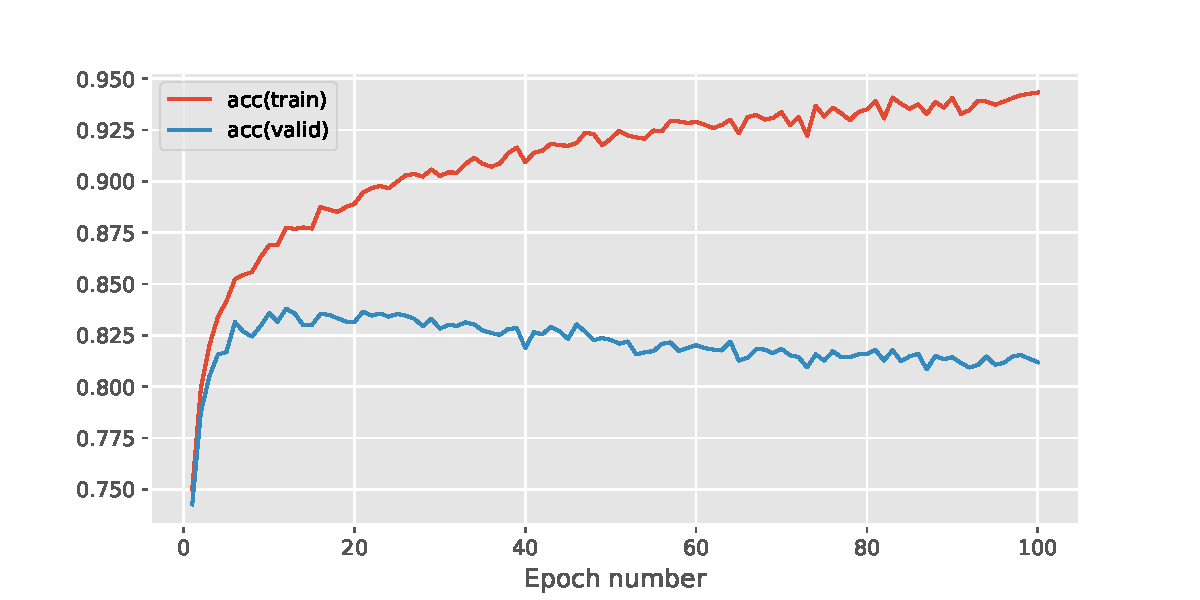
\includegraphics[width=\columnwidth]{e.pdf}}
\caption{Accuracy of models with Adam learning rule. \n
Accuracy of train dataset:0.943 \n
Accuracy of valid dataset:0.812
}
\end{center}
\vskip -5mm
\end{figure}

The result shows that these learning rules improves the accuracy of prediction of training and validation dataset. However, the differnece goes up, and this means that overfitting happens. It may be solved by dropout technique.

% You should, in your own words, explain what the different learning rules do, and how they differ.  You should then present your experiments and results, comparing and contrasting stochastic gradient descent, RMSProp, and Adam.  As before concentrate on the ``what'' (remember give enough information so someone can reproduce your experiments), the ``why'' (why did you choose the experiments that you performed -- you may have been motivated by your earlier results, by the literature, or by a specific research question), and the interpretation of your results.
%
% In every section, you should present your results in a way that makes it easy for a reader to understand what they mean. You should facilitate comparisons either using graphs with multiple curves or (if appropriate, e.g. for accuracies) a results table. You need to avoid having too many figures, poorly labelled graphs, and graphs which should be comparable but which use different axis scales. A good presentation will enable the reader to compare trends in the same graph -- each graph should summarise the results relating to a particular research (sub)question.
%
% Your discussion should interpret the results, both in terms of summarising the outcomes of a particular experiment, and attempting to relate to the underlying models. A good report would have some analysis, resulting in an understanding of why particular results are observed, perhaps with reference to the literature. Use bibtex to organise your references -- in this case the references are in the file \verb+example-refs.bib+.  Here is a an example reference \citep{langley00}.

\section{Batch normalisation}
In this secion, we present Batch normalization.

Covariate shift in machine learning means that the distribution of input data deviates, and it makes the algorithms hard to predict.
In deep neural network, the distribution of input in each activation goes diffenrent, and this is called internal convariate shift.
It is known that the whitening technique, which makes the varidation to 1 and average to 0, makes the converge of neural netowrk faster. Before this technique, normalization and standardization is used in the pre-processing of data.
Batch normalization is presented by Ioffe and Szegedy in 2015. This method normalize the inputs in each activation. Not only dataset but also all inputs is whitened, therefore, it control internal convariate shift and converge goes faster.

We implement batch to the baseline model with SGD, RMSProp and Adam optimizer.
The result is on figure 6 to 8 and table 2.
\begin{figure}[h]
\vskip 5mm
\begin{center}
\centerline{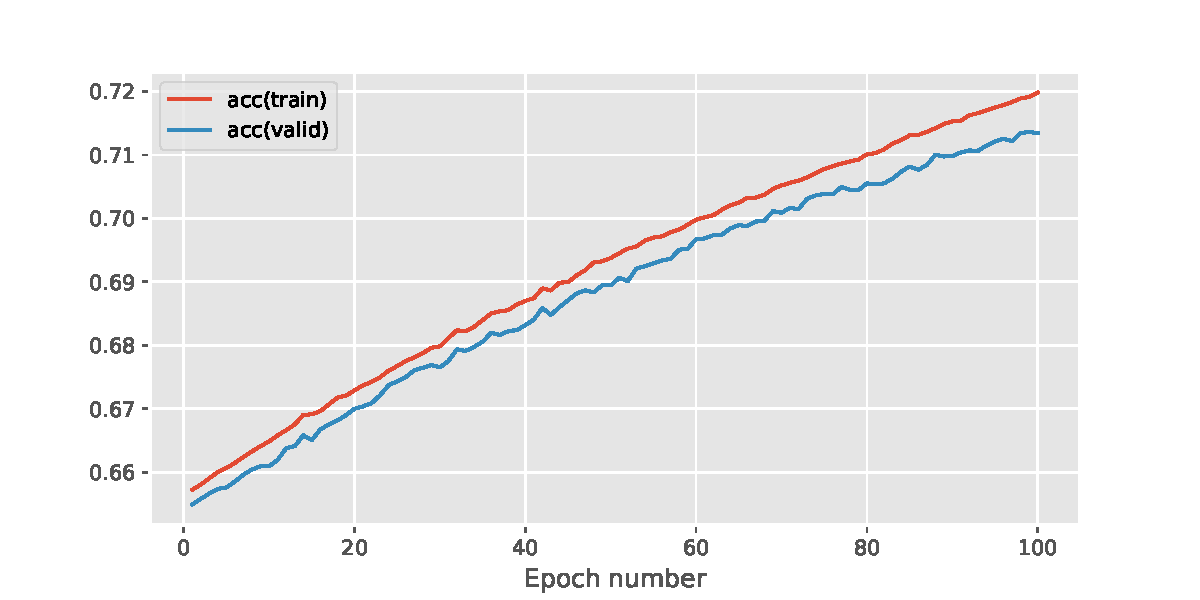
\includegraphics[width=\columnwidth]{f.pdf}}
\caption{Accuracy of models with Batch and SGD. \n
Accuracy of train dataset:0.720 \n
Accuracy of valid dataset:0.713
}
\end{center}
\vskip -5mm
\end{figure}

\begin{figure}[h]
\vskip 5mm
\begin{center}
\centerline{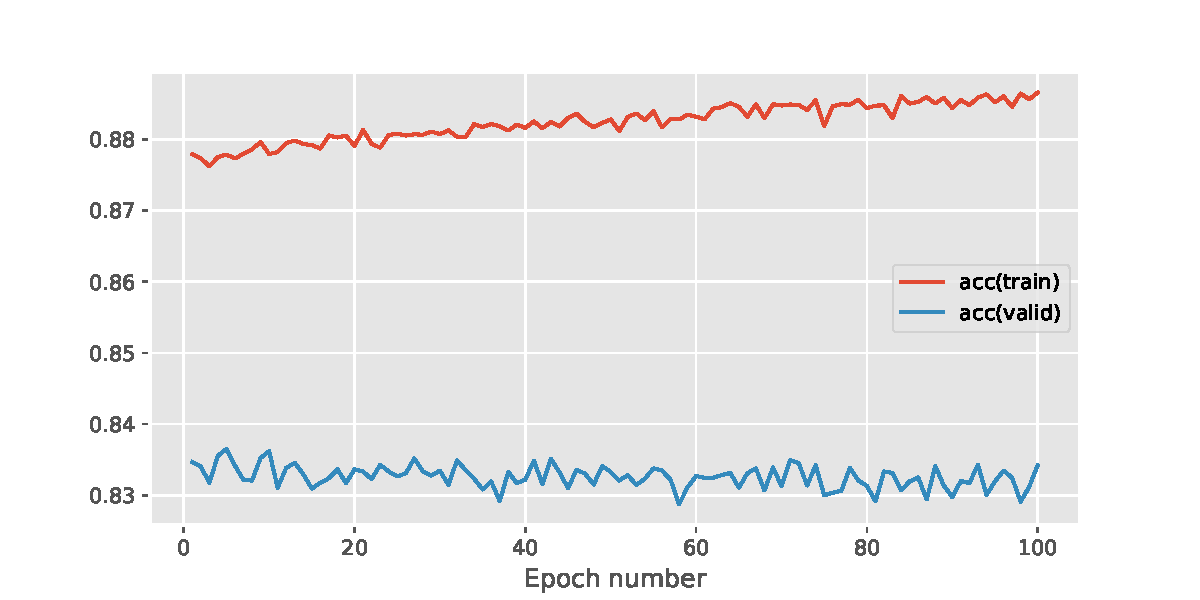
\includegraphics[width=\columnwidth]{g.pdf}}
\caption{Accuracy of models with Batch and RMSProp. \n
Accuracy of train dataset:0.887 \n
Accuracy of valid dataset:0.834
}
\end{center}
\vskip -5mm
\end{figure}

\begin{figure}[h]
\vskip 5mm
\begin{center}
\centerline{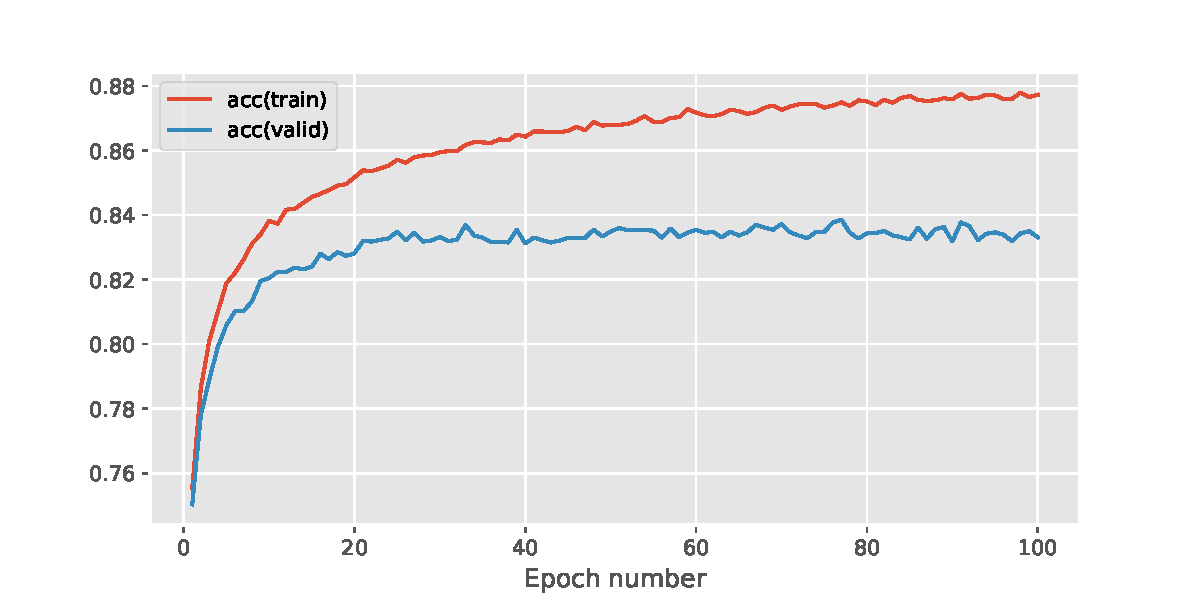
\includegraphics[width=\columnwidth]{h.pdf}}
\caption{Accuracy of models with Batch and Adam. \n
Accuracy of train dataset:0.877 \n
Accuracy of valid dataset:0.833
}
\end{center}
\vskip -5mm
\end{figure}

\begin{table}[h]
\vskip 3mm
\begin{center}
\begin{small}
\begin{sc}
\begin{tabular}{lcccr}
\hline
\abovespace\belowspace
&acc(train) & acc(val) & error(train) & error(val) \\
\hline
\abovespace
SGD     & 0.737      & 0.733           & 0.919        & 0.936             \\ \hline
RMSProp & 0.944      & 0.809           & 0.135        & 1.37              \\ \hline
Adam    & 0.943      & 0.812           & 0.138        & 1.20              \\
\hline
SGD + Batch & 0.720 & 0.713           & 0.969        & 0.979               \\
\hline
RMSProp + Batch & 0.878  &0.834     & 0.354      & 0.542                     \\
\hline
Adam + Batch & 0.877 & 0.833        & 0.323     & 0.507                 \\
\hline
\end{tabular}
\end{sc}
\end{small}
\caption{Accuracy and mean square error of models with three different learning rules and batch normalization.}
\label{tab:sample-table}
\end{center}
\vskip -3mm
\end{table}
% In this section you should present batch normalisation,  supported using equations or algorithmic pseudocode.  Following this present your experiments, again remembering to include the ``what'', the ``why'', and the interpretation of results.
The accuracy in RMSProp and Adam improves, and it controls overfitting. Although the model with SGD does not change dynamically, batch normalization is beneficial.

Finally for this section, we implement baseline model with dropout, adam and batch normalization.
The result in on Figure 9. Although the acuuracy worsened, the overfitting improves.

\begin{figure}[h]
\vskip 5mm
\begin{center}
\centerline{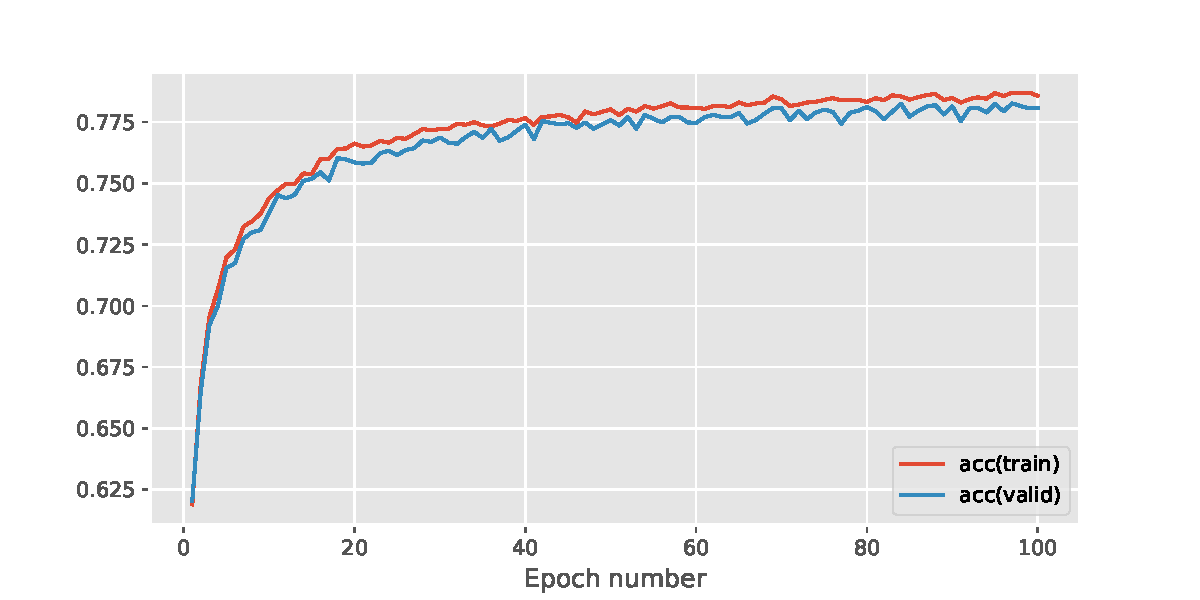
\includegraphics[width=\columnwidth]{i.pdf}}
\caption{Accuracy of models with Batch and Adam. \n
Accuracy of train dataset:0.786 \n
Accuracy of valid dataset:0.781
}
\end{center}
\vskip -5mm
\end{figure}


\section{Convolutional networks}
In this section, we present Convolution Neural Network (CNN).

CNN is constructed with convolution layer and pooling layer.
Before CNN, we use inputs data as one dimension. However, it ignores the spatial structure of the input images, and it is weak to learn the same features at different places in the input image.
Convolution layer has a filter with shared weight. To apply the filter to the image create reduced feature map.
Pooling layer is applied after convolution layer. Pooling layer reduces information to appropriate data size. In this experiment, we use max pooling layer. Max pooling takes the maximum value of the units in the region. This layer reduces the cost of computation, controls overfitting, and makes the model robust to precise displacement.

We construct three models. The first model containes one convolution and maxpooling model (Figure 10). The second model containes two convolution and mmaxpooling layers. These are based on baseline model, and the learning rule is SGD, learning rate in 0.001.

The third model is based on the paper Ioffe and Szegedy in 2015. It containes three convolution and max pooling layers, and two batch normalization layers. The activation function is hyperbolic tangent, and the learning rate is 0.03(Algorithm 1).

The epoch size is 50 in this experiment because CNN takes huge computation cost. It takes 48 hours for third model to learn train dataset.
The result is on Figure 11 to 13 and table 3.

\begin{figure}[h]
\vskip 5mm
\begin{center}
\centerline{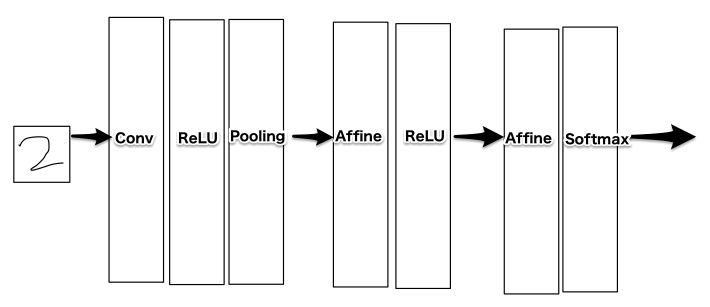
\includegraphics[width=\columnwidth]{j.png}}
\caption{The First Model.
}
\end{center}
\vskip -5mm
\end{figure}

\begin{algorithm}[h]
\begin{algorithmic}
      \STATE ReshapeLayer((1,28,28,)) \\
      \STATE ConvolutionalLayer(1, 5, 28, 28, 5, 5) \\
      \STATE TanhLayer() \\
      \STATE MaxPoolingLayer()  \\
      \STATE ConvolutionalLayer(5,10,12,12,5,5) \\
      \STATE TanhLayer() \\
      \STATE ConvolutionalLayer(10,20,8,8,5,5) \\
     \STATE TanhLayer() \\
      \STATE ReshapeLayer((320,)) \\
      \STATE BatchNormalizationLayer(320) \\
      \STATE ReshapeLayer((20, 4, 4,)) \\
      \STATE MaxPoolingLayer() \\
      \STATE ReshapeLayer((80,)) \\
      \STATE BatchNormalizationLayer(80) \\
      \STATE AffineLayer(80, $output_{dim}$, $weights_{init}$, $biases_{init}$) \\
\end{algorithmic}
  \caption{The Third Model}
  \label{alg:example}
\end{algorithm}

\begin{table}[h]
\vskip 3mm
\begin{center}
\begin{small}
\begin{sc}
\begin{tabular}{lcccr}
\hline
\abovespace\belowspace
&acc(train) & acc(val) & error(train) & error(val) \\
\hline
\abovespace
First Model     & 0.716      & 0.710           & 1.00        & 1.01             \\ \hline
Second Model & 0.743      & 0.745          & 0.852       & 0.847              \\ \hline
Third Model    & 0.870      & 0.853          & 0.373        & 0.432              \\
\hline
\end{tabular}
\end{sc}
\end{small}
\caption{Accuracy and mean square error of three models with CNN}
\label{tab:sample-table}
\end{center}
\vskip -3mm
\end{table}

\begin{figure}[h]
\vskip 5mm
\begin{center}
\centerline{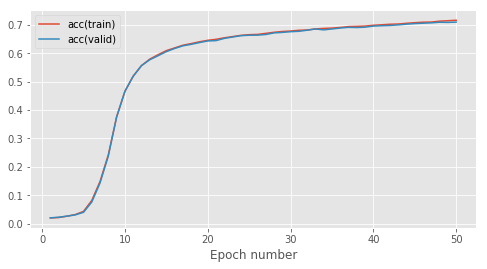
\includegraphics[width=\columnwidth]{k.jpg}}
\caption{Accuracy of the first model. \n
Accuracy of train dataset:0.716 \n
Accuracy of valid dataset:0.710
}
\end{center}
\vskip -5mm
\end{figure}

\begin{figure}[h]
\vskip 5mm
\begin{center}
\centerline{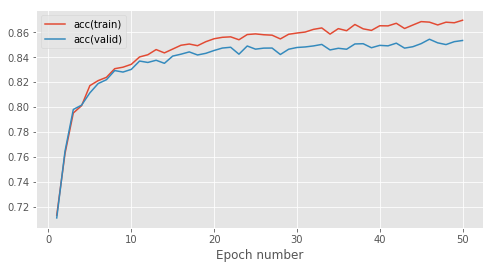
\includegraphics[width=\columnwidth]{m.jpg}}
\caption{Accuracy of the third model. \n
Accuracy of train dataset:0.743 \n
Accuracy of valid dataset:0.745
}
\end{center}
\vskip -5mm
\end{figure}

\begin{figure}[h]
\vskip 5mm
\begin{center}
\centerline{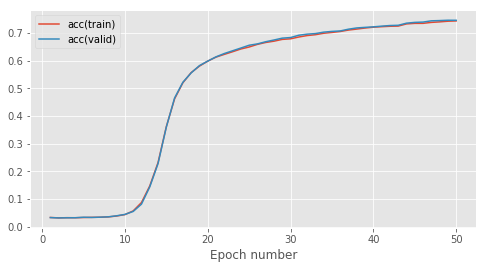
\includegraphics[width=\columnwidth]{l.jpg}}
\caption{Accuracy of the second model. \n
Accuracy of train dataset:0.870\n
Accuracy of valid dataset:0.853
}
\end{center}
\vskip -5mm
\end{figure}

As a result, CNN improves the accuracy and reduces train error. The combination of batch normalization and CNN improves the performance.

% In this section you should present your experiments with convolutional networks.  Explain the idea of convolutional layers and pooling layers, and briefly explain how you did the implementation.  There is no need to include chunks of code.  You should report the experiments you have undertaken, again remembering to include \emph{what} experiments you performed (include details of hyperparameters, etc.),  \emph{why} you performed them (what was the motivation for the experiments, what research questions are you exploring), and the interpretation and discussion of your results.

\section{Test results}
% The results reported in the previous sections should be on the validation set.  You should finally report results on the EMNIST test set using what you judge to the be the best deep neural network (without convolutional layers) and the best convolutional network.  Again focus on what the experiments were (be precise), why you chose to do them (in particular, how did you choose the architectures/settings to use with the test set), and a discussion/interpretation of the results.
In total, the third model in section 5 marks the highest performance. However, we could not test the model on test set because of time. However, we can say that the CNN model marks great performance, but deep neuralnetwork with batch normalization have a potential to approach thier performance.


\section{Conclusions}
\label{sec:concl}
In this coursework, we could prove that batch normalization, and CNN improves the neural network. These techniques solve various problems, for example, internal convariate shift, location information of inputs, and so on. We realize that the combination of CNN and batch marks impressive performance.

The problem is that the computational cost is enormous, especially CNN. We cannot imagine how can solve that problem. However, this problem is the critical topics in this field.% \bibliography{example-refs}
%
\end{document}


% This document was modified from the file originally made available by
% Pat Langley and Andrea Danyluk for ICML-2K. This version was
% created by Lise Getoor and Tobias Scheffer, it was slightly modified
% from the 2010 version by Thorsten Joachims & Johannes Fuernkranz,
% slightly modified from the 2009 version by Kiri Wagstaff and
% Sam Roweis's 2008 version, which is slightly modified from
% Prasad Tadepalli's 2007 version which is a lightly
% changed version of the previous year's version by Andrew Moore,
% which was in turn edited from those of Kristian Kersting and
% Codrina Lauth. Alex Smola contributed to the algorithmic style files.
